% Chapter 1

\chapter{Phương pháp phần tử hữu hạn giải bài toán biến dạng đàn hồi}\label{Chapter1}
\renewcommand{\baselinestretch}{1.25}
\minitoc
\renewcommand{\baselinestretch}{1.5}
Trong chương này, ta sẽ trình bày một lược đồ giải số cho bài toán biến dạng đàn hồi. Phần đầu tiên, một vài kiến thức cơ sở. Phần \ref{sec:chap1_problem} phát biểu phương trình biến dạng đàn hồi. Phần \ref{sec:chap1_characteristicMethod} dẫn dắt đưa bài toán ban đầu về dưới dạng biến phân. Phương pháp phần tử hữu hạn sẽ được sử dụng để rời rạc hóa không gian trong phần \ref{sec:chap1_spatialDiscrete}. Phần tiếp theo \ref{sec:chap1_linearSystem} trình bày cách xây dựng hệ phương trình tuyến tính rời rạc. Và cuối cùng là một vài ví dụ của bài toán trong công nghiệp vật liệu.

%----------------------------------------------------------------------------------------
\section{Cơ sở toán học}
\subsection{Không gian Hilbert}
\begin{defi}
Không gian vectơ $V$ trên trường vô hướng $K$ là một tập các vectơ, trong đó có xác định hai phép toán:
\begin{itemize}
\item Phép cộng: ứng với mỗi cặp $x, y \in V$ xác định được phần tử thuộc $V$ viết là $x+y$.
\item Phép nhân vô hướng: với mỗi phần tử $x \in V$ và số $k \in \mathbb{R}$, xác định được một phần tử thuộc $V$, viết là $kx$ (hay $xk$);
\end{itemize}
sao cho thỏa mãn 8 tính chất sau:
\begin{itemize}
\item $x+y=y+x, \forall x,y\in V$
\item $x+(y+z)=(x+y)+z, \forall x,y,z\in V$
\item $\exists \theta \in V: \theta +x=x+\theta =x, \forall x\in V$ (phần tử trung hòa hay phần tử không)
\item $\forall x\in V \exists -x \in V : x + (-x) = -x + x=\theta$ (phần tử đối)
\item $k(x+y) = kx+ky, \forall x,y\in V, \forall k\in\mathbb{R}$
\item $(k+l)x = kx + lx, \forall x\in V, \forall k,l\in\mathbb{R}$
\end{itemize}
\end{defi}
\begin{defi}
Không gian định chuẩn là một không gian vectơ $V$ trong đó mỗi phần tử $x\in V$ đều xác định một số thực ký hiệu là $||x||$, gọi là chuẩn của $x$, thỏa mãn 3 tính chất sau:
\begin{itemize}
\item $||x|| \geq 0, \forall x\in V;||x|| = 0 \leftrightarrow x=\theta$
\item $||kx||=|k|.||x||,\forall x\in V, \forall k\in \mathbb{R}$
\item $||x+y||\leq ||x||+||y||,\forall x,y \in V$
\end{itemize}
\end{defi}
Tập các phần tử của không gian vectơ $V$ gọi là tập nền của không gian chuẩn $V$.
\subsection{Một số không gian hàm}
\subsection{Phiếm hàm trong không gian Hilbert}
\subsection{Bài toán yếu trong không gian Hilbert}
\section{Phương trình đàn hồi}\label{sec:chap1_problem}
Cho $\Om$ là miền trong không gian $\R^d (d=2 \text{ hoặc } 3)$ có biên $\Gamma = \{\Gamma_D, \Gamma_N\}$. $\Gamma_D$ là điều kiện biên Dirichlet, $\Gamma_N$ là điều kiện biên Neumann. Đặt u là chuyển vị của một tấm được cấu tạo vật liệu khác nhau. Mối quan hệ giữa hệ số biến dạng và chuyển vị của tấm được đưa ra bởi: % ????
$$e(u) = (\nabla u + \nabla u^t)/2$$

Giả sử rằng vật liệu có tính đàn hồi tuyến tính và đẳng hướng; và rằng các chuyển vị là nhỏ, định luật Hooke đưa ra mối quan hệ giữa hệ số đàn hồi và hệ số biến dạng:
\begin{equation}\label{equa1}
\mathcal{A}e(u) = 2\mu e(u) + \lambda Tr(e(u))Id
\end{equation}
trong đó:
\begin{itemize}
\item $\mathcal{A}e(u)$ là hệ số đàn hồi,
\item $Id$ là ma trận đơn vị,
\item $Tr(.)$ là vết,
\item $\lambda, \mu$ là các hệ số mô tả các tính chất cơ học của vật và và bản thân chúng có liên quan đến hằng số được biết đến nhiều hơn là hằng số mô-đun đàn hồi Young $E$ và hệ số Poisson $v$:
$$\mu = \frac{E}{2(1 + v)}, \qquad \lambda = \frac{Ev}{(1 + v)(1 - 2v)}.$$
\end{itemize}

Ta định nghĩa $g$ là ngoại lực tác động bên ngoài, $f$ là trọng lực của vật. Ta có hệ phương trình tuyến tính đàn hồi:
\begin{equation}\label{prob}
\quad\quad\quad\quad\quad
\begin{cases}
-\text{div}(\mathcal{A}e(u)) = f \qquad \text{trong } \Omega,\\
u = 0 \quad\qquad\qquad\qquad \text{trên } \Gamma_D, \\
\mathcal{A}e(u))n = g \qquad\qquad \text{trên } \Gamma_N.
\end{cases}
\end{equation}

\section{Công thức biến phân của bài toán biến dạng đàn hồi}\label{sec:chap1_characteristicMethod}
Như đã thảo luận trong phần trước, việc biến đổi bài toán mô tả các vấn đề cơ học (strong form) về bài toán dạng yếu (weak form) hay bài toán biến phân là một bước quan trọng của phương pháp phần tử hữu hạn. Do đó, trong phần này, ta sẽ nghiên cứu dạng biến phân của hệ phương trình tuyến tính đàn hồi \eqref{prob}.\\

Ký hiệu $V$ là không gian hàm của chuyển vị $u$. Gọi $v \in V$ là hàm thử. Nhân cả hai vế phương trình đầu tiên của hệ \eqref{prob} với hàm thử $v$ rồi lấy tích phân trên miền $\Omega$, ta được:
$$-\int_\Omega\text{div}(\mathcal{A}e(u)).v = \int_\Omega f.v$$
Áp dụng công thức Green:
$$\int_\Omega\mathcal{A}e(u).\nabla v - \int_{\partial \Omega}(\mathcal{A}e(u)n) = \int_\Omega f.v.v,$$
$$\int_\Omega\mathcal{A}e(u).\nabla v = \int_\Omega f.v + \int_{\partial \Omega}(\mathcal{A}e(u)n).v$$
Ta định nghĩa $a : b = \sum_{ij}{a_{ij}b_{ij}}.$ Không gian hàm thử $V$ được chọn sao cho hàm thử $v \in V$ bị triệt tiêu trên phần biên đặt điều kiện Dirichlet, nghĩa là:
$$V = H^1_{\Gamma_D}(\Omega)^d := \{v \in H^1(\Omega)^d : v = 0|\Gamma_D\}.$$
Kết hợp với điều kiện biên Neumann của hệ \eqref{prob}, ta có thể viết lại:
$$\int_\Omega\mathcal{A}e(u):e(v) = \int_\Omega f.v + \int_{\Gamma_N}g.v$$
Thay \eqref{equa1} vào ta được:
$$\int_\Omega(2\mu e(u) + \lambda Tr(e(u))Id):e(v) = \int_\Omega f.v + \int_{\Gamma_N}g.v$$
$$\int_\Omega 2\mu e(u) : e(v) + \lambda(\text{div}u)(\text{div}v) = \int_\Omega f.v + \int_{\Gamma_N}g.v.$$\\
Bài toán biến dạng đàn hồi có thể viết dưới dạng yếu tương đương: tìm $u\in V$ thỏa mãn:
\begin{equation}\label{prowf}
a(u,v) = L(v)
\end{equation}
Trong đó :
$$a(u,v) = \int_\Omega 2\mu e(u) : e(v) + \lambda(\text{div}u)(\text{div}v)$$
$$L(v) = \int_\Omega f.v + \int_{\Gamma_N}g.v$$
Sự tồn tại và duy nhất nghiệm của bài toán yếu \ref{prowf} của bài toán đàn hồi được chứng minh dựa theo định lý Lax-Milgram.
\begin{thm}[Định lý Lax-Milgram]\label{thm:chap1_reducedVariationalForm}
Cho $a(.,.)$ là dạng song tuyến tính bị chặn trên $V$ và là V-elliptic. $L(.)$ là phiếm hàm tuyến tính bị chặn trên $V$. Khi đó bài toán yếu \ref{prowf} có nghiệm và nghiệm đó là duy nhất.
\end{thm}
\section{Dạng rời rạc của bài toán}
Sử dụng xấp xỉ phần tử hữu hạn, không gian hàm thử $V$ được thay thế bằng một không gian con hữu hạn chiều $V_N$. Dạng rời rạc không gian tương ứng của bài toán \ref{prowf}: Tìm $u_h \in V_N$
sao cho $u_h = 0$ trên $\Gamma_D$ và với mọi $v_h \in V_N$ với $v_h = 0$ trên $\Gamma_D$,
\begin{equation}\label{prod}
\int_\Omega 2\mu e(u_h) : e(v_h) + \lambda(\text{div}u_h)(\text{div}v_h) = \int_\Omega f.v_h + \int_{\Gamma_N}g.v_h
\end{equation}
\section{Hệ phương trình tuyến tính rời rạc}\label{sec:chap1_linearSystem}
Gọi $\mathcal{T}$ là tập các tam giác của $\Omega$ sau khi rời rạc hóa. Gọi $\mathcal{N}$ là tập tất cả các nút của $\mathcal{T}$; Tập $(\eta_k,...,\eta_{dN})=(\varphi_1e_1, \varphi_2e_2,...,\varphi_1e_d,...,\varphi_Ne_1,\varphi_Ne_2,...,\varphi_Ne_d)$ là tập các nút cơ sở của không gian con hữu hạn chiều $V_N$, trong đó $N$ tổng số đỉnh của lưới, $d$ là số chiều của vec-tơ chuyển vị, và $\varphi_i$ là hàm mũ tại đỉnh $x_i$ trong tam giác $\mathcal{T}$:
$$\varphi_{x_i}(x_j) = \begin{cases}
1 \text{ with } x_i = x_j, \\
0 \text{ with } x_i \neq x_j.
\end{cases}$$
Áp dụng điều kiện biên với $i = 1,...,dN$, ta được:
$$\int_\Omega 2\mu e(u_h) : e(\eta_i) + \lambda(\text{div}u_h)(\text{div}\eta_i) = \int_\Omega f.\eta_i + \int_{\Gamma_N}g.\eta_i.$$
Khi đó, véc-tơ chuyển vị được viết lại dưới dạng: $u_h = \sum_{j=1}^{dN}U_i\eta_i$. Từ đó ta có được hệ phương trình tuyến tính:
$$\displaystyle\sum^{dN}_{i=1}(\displaystyle\int_\Omega 2\mu e(\eta_j) : e(\eta_i) + \lambda(\text{div}\eta_j)(\text{div}\eta_i)) = \int_\Omega f.\eta_i + \int_{\Gamma_N}g.\eta_i.$$
Ký hiệu $A=(A_{ij})\in\mathbb{R}^{dN x dN}$, trong đó:
$$A_{ij}=\displaystyle\int_\Omega 2\mu e(\eta_j) : e(\eta_i) + \lambda(\text{div}\eta_j)(\text{div}\eta_i),$$
Ma trận $A$ còn được gọi là ma trận đô cứng (stiffness matrix).
Ký hiệu ma trận vế phải $B=(b_i)\in\mathbb{R}^{dN}$, trong đó:
$$b_i=\int_\Omega f.\eta_i + \int_{\Gamma_N}g.\eta_i.$$
Ta thu được hệ phương trình đại số tương ứng của bài toán đàn hồi \eqref{prob}:
\begin{equation}\label{pron}
Au=B
\end{equation}
Ma trận độ cứng $A$ là ma trận thưa, đối xứng và nửa xác định dương.
\section{Các ví dụ mô phỏng số}
Trong phần này, ta sẽ minh họa các ví dụ mô phỏng số cho hệ phương trình tuyến tính đàn hồi. Hầu hết các thí nghiệm sẽ được tiến hành trong không gian $d=2$ chiều. Riêng ví dụ cuối là mô phỏng biến dạng trong $d=3$ chiều.\\
Mã nguồn chương trình và một số thí nghiệm giải số cho các bài toán biến dạng đàn hồi có thể tìm thấy tại địa chỉ: \url{https://github.com/}. Tác giả luôn mong muốn nhận được những đề xuất, đóng góp cho việc phát triển mã nguồn và các thí nghiệm mô phỏng số.
\subsection{Thứ nguyên}
\subsection{Lực kéo}
Trong phần này, ta sẽ trình bày các kết quả mô phỏng số cho bài toán liên quan đến lực kéo đàn hồi.\\
Cho một tấm kim loại có một lỗ ở giữa chịu lực kéo $F=[0,1e4]$ tại $x=0.4$ và trọng lực $g=(0,-9.81)$ với hằng số mô-đun đàn hồi Young $E=7e4$ và hệ số Poisson $v=0,3$ \cite{TIT-07}. Khởi tạo lưới với 1607 tam giác \eqref{fig:exam21}.\\
\begin{figure}[http]
\centering
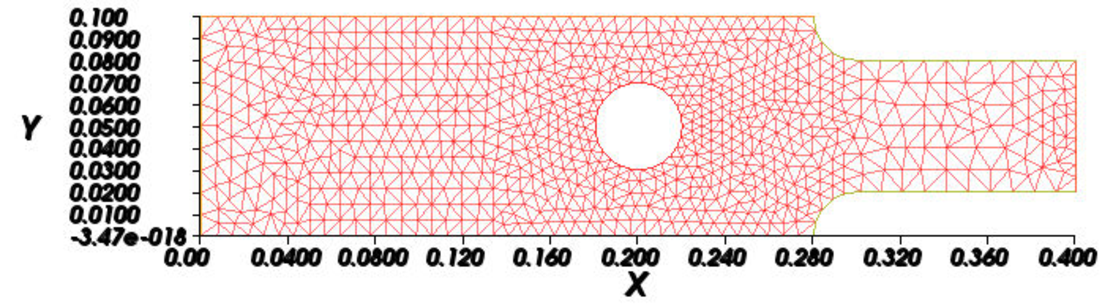
\includegraphics[width=1\textwidth]{paper/4-2-1.pdf}
\caption{Trạng thái ban đầu của tấm kim loại.}
\label{fig:exam21}
\end{figure}\\
Hình dưới đây cho thấy sự biến dạng của tấm kim loại chịu một lực kéo $F = 100$. Do lực kéo là rất nhỏ nên độ biến dạng của tấm kim loại là không lớn \eqref{fig:exam22}.\\
\begin{figure}[http]
\centering
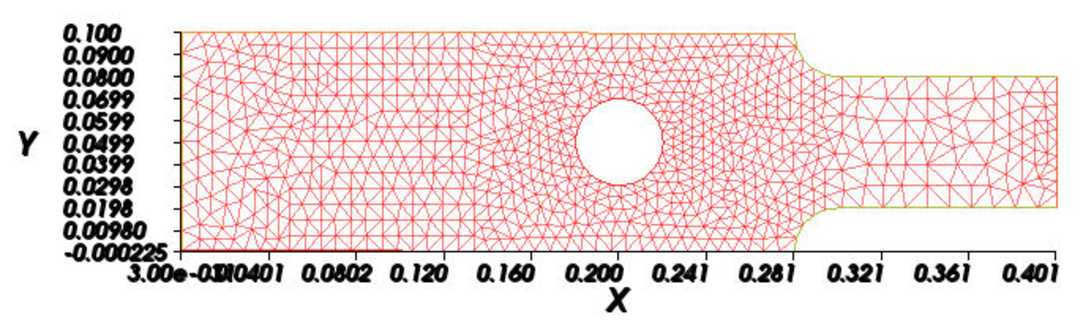
\includegraphics[width=1\textwidth]{paper/4-2-2.pdf}
\caption{Tấm kim loại dưới tác dụng của lực kéo F=100.}
\label{fig:exam22}
\end{figure}\\
Khi ta tăng lực kéo F lên F=5e3 (hình \ref{fig:exam23}) và F=1e4 (hình \ref{fig:exam24}) thì ta thấy độ biến dạng rõ hơn.\\
\begin{figure}[http]
\centering
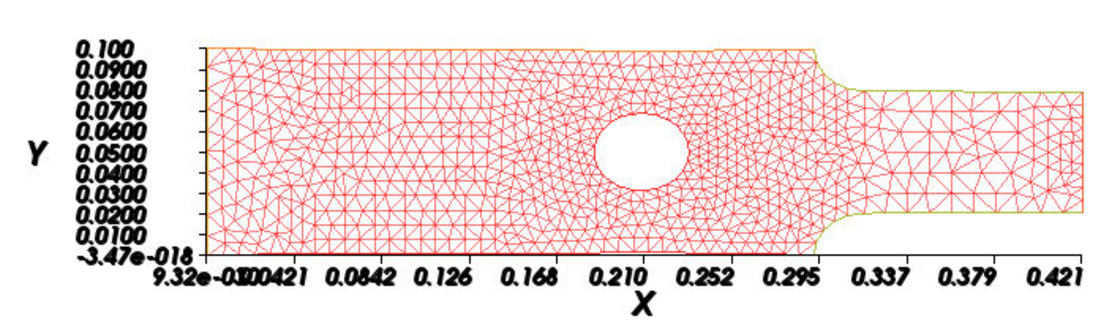
\includegraphics[width=1\textwidth]{paper/4-2-3.pdf}
\caption{Tấm kim loại dưới tác dụng của lực kéo F=5e3.}
\label{fig:exam23}
\end{figure}
\begin{figure}[http]
\centering
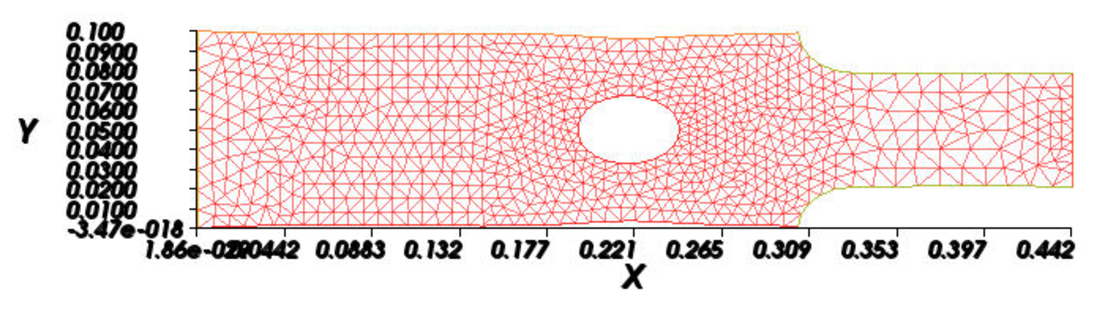
\includegraphics[width=1\textwidth]{paper/4-2-4.pdf}
\caption{Tấm kim loại dưới tác dụng của lực kéo F=1e4.}
\label{fig:exam24}
\end{figure}
\subsection{Lực nén}
Xét một tấm kim loại có một lỗ ở giữa chịu tác động của một lực nén $f=(-1e4,0)$ và trọng lực $g=(0,-9.81)$. Cho hằng số mô-đun đàn hồi Young $E=7e4$ và hệ số Poisson $v=0,3$ \cite{TIT-07}. Ta có hình \eqref{fig:exam31} - khởi tạo lưới ban đầu của tấm kim loại và hình \eqref{fig:exam32} - thể hiện lưới biến dạng của tấm kim loại sau khi chịu tác động bởi lực nén.\\
\begin{figure}[http]
\centering
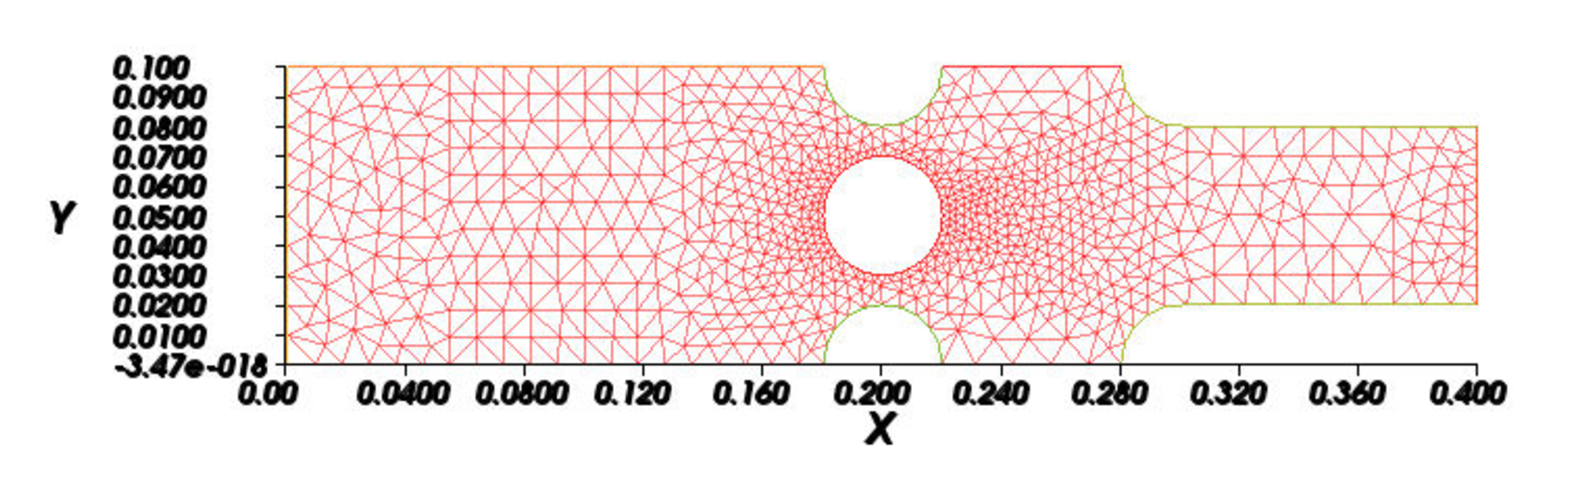
\includegraphics[width=1\textwidth]{paper/4-3-1.pdf}
\caption{Tấm kim loại ở trạng thái ban đầu.}
\label{fig:exam31}
\end{figure}
\begin{figure}[http]
\centering
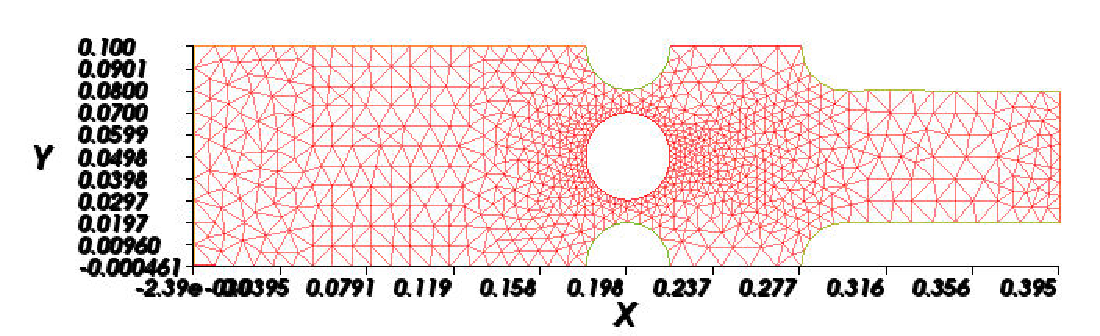
\includegraphics[width=1\textwidth]{paper/4-3-2.pdf}
\caption{Tấm kim loại dưới tác dụng của lực nén.}
\label{fig:exam32}
\end{figure}\\

Xét một tấm kim loại có kích thước là $2 * 2$ với đáy cố định, chịu tác dụng của một lực nén $f = 1e7$ lên phía trên của tấm kim loại. Tấm kim loại có một lỗ được cho bởi phương trình $r = 0.5 + 0.2 sin(kt)$ trong tọa độ cực. Trong ví dụ này, ta xét $k=5$. Cho hằng số mô-đun đàn hồi Young và hệ số Poisson lần lượt bằng $E=1e9, v=0,3$. Dưới đây là lưới khởi tạo với 5796 tam giác của tấm kim loại \ref{fig:exam33}:\\

\begin{figure}[http]
\centering
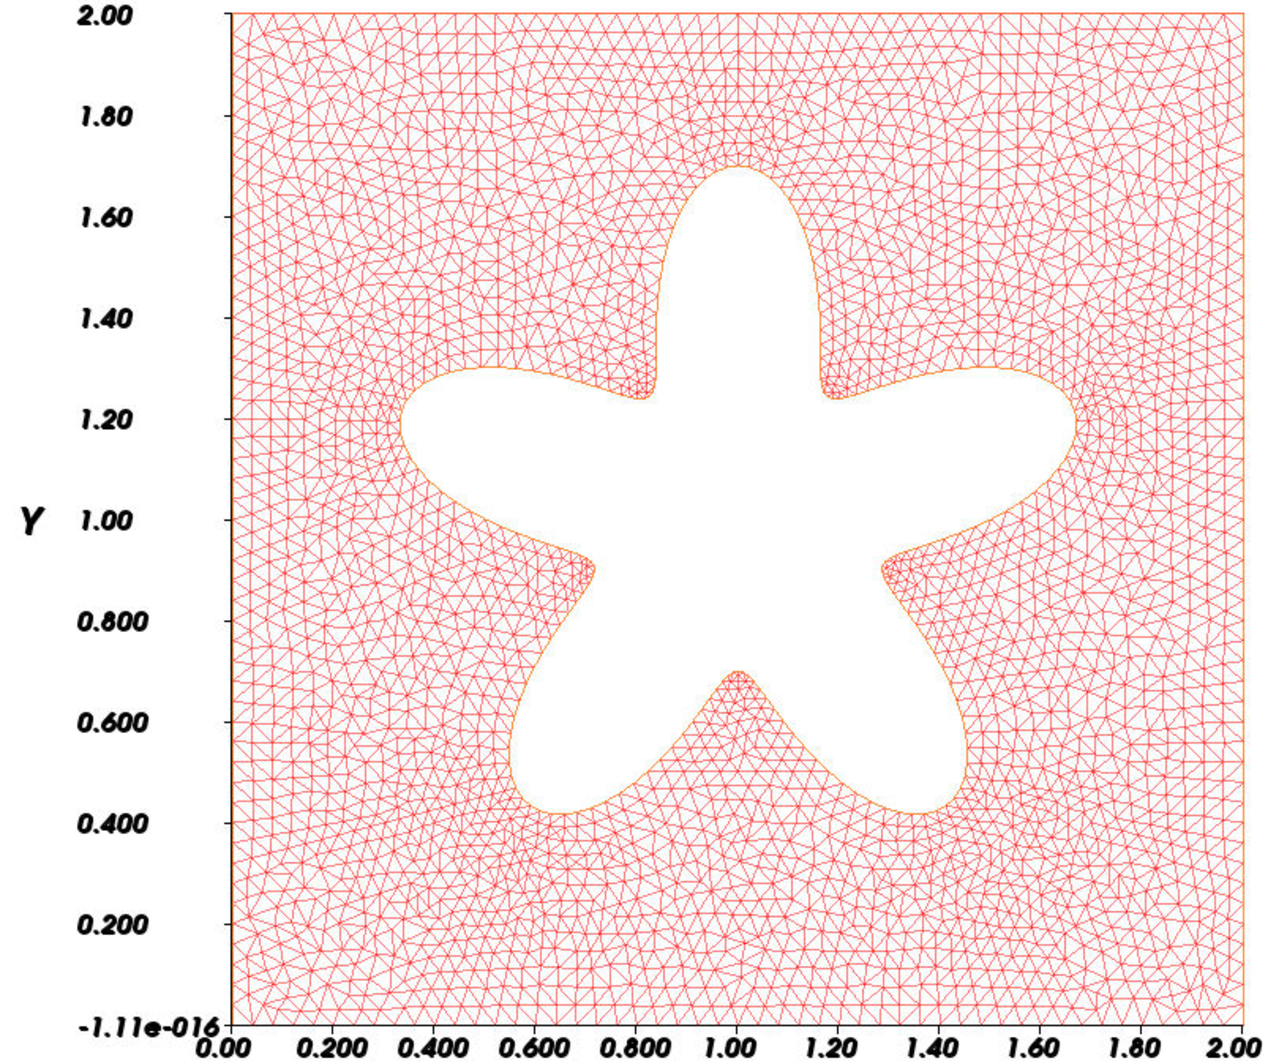
\includegraphics[width=0.6\textwidth]{paper/4-3-3.pdf}
\caption{Tấm kim loại $2 * 2$ với lỗ $r = 0.5 + 0.2 sin(kt)$.}
\label{fig:exam33}
\end{figure}
Dưới tác dụng của lực nén, tấm sẽ bị nén theo chiều y và phình to ra theo hướng x. Hình sau biểu thị sự dịch chuyển biến dạng của tấm kim loại:\\
\begin{figure}[http]
\centering
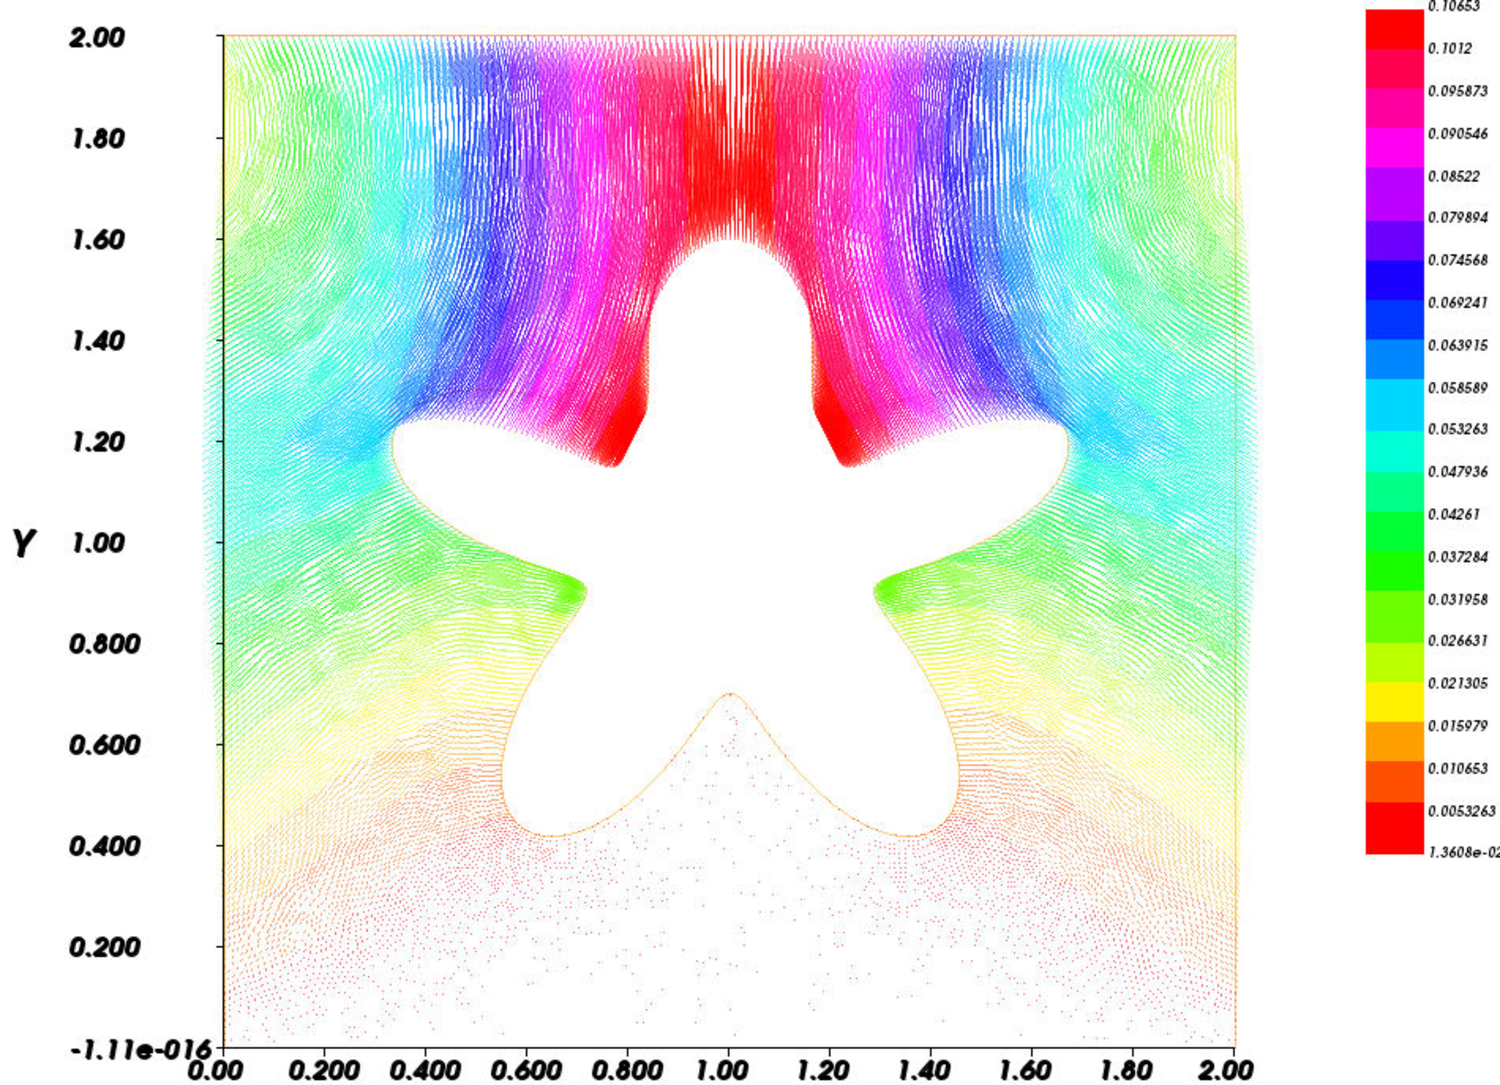
\includegraphics[width=0.6\textwidth]{paper/4-3-4.pdf}
\caption{Hướng dịch chuyển của tấm kim loại.}
\label{fig:exam34}
\end{figure}\\
\begin{figure}[http]
\centering
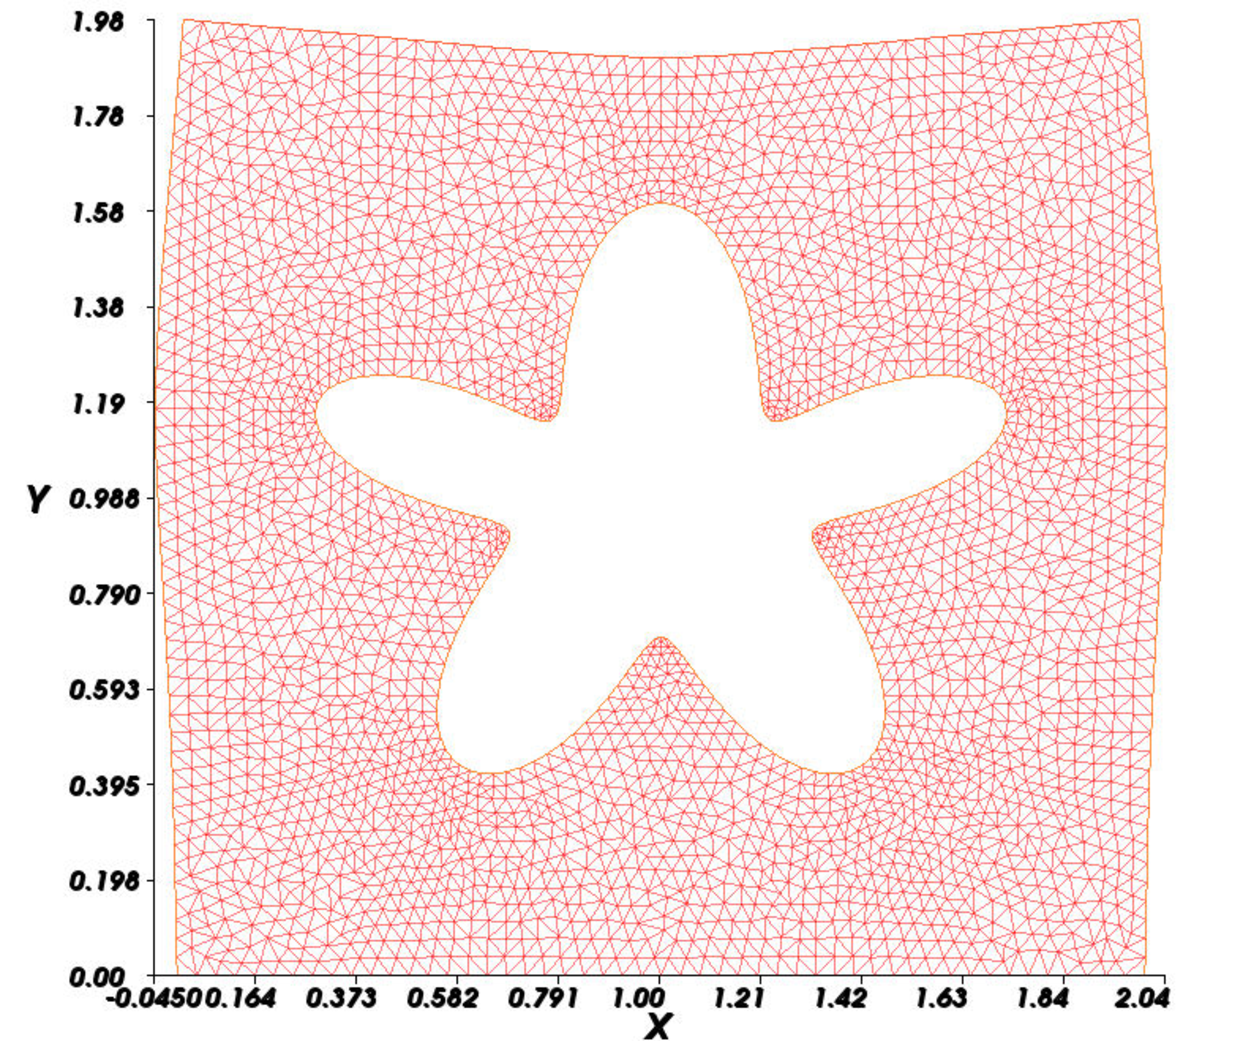
\includegraphics[width=0.6\textwidth]{paper/4-3-5.pdf}
\caption{Tấm kim loại sau khi bị biến dạng.}
\label{fig:exam35}
\end{figure}\\
\subsection{Áp suất}
Một tấm kim loại hình khuyên phải chịu một áp lực bên trong như hình \ref{fig:exam41} với $p=1e3,E=2e5, v=0.3, r_i=42, r_e=50, h=1 (h<<r_i)$ \cite{TIT-07}. Do $(h<<r_i)$ nên ta có thể coi đây là một bài toán 2 chiều. Ở ví dụ tiếp theo, ta xét một ống kim loại có cùng $p, E, v, r_i, r_e$ với chiều dài không nhỏ hơn quá nhiều so với bán kính của ống. Khi đó, bài toán trở thành bài toán 3 chiều.\\
\begin{figure}[http]
\centering
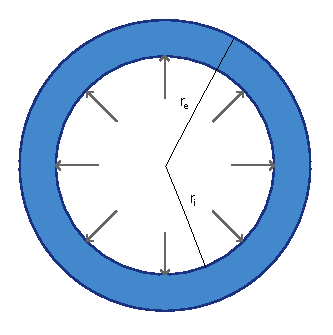
\includegraphics[width=0.5\textwidth]{paper/4-4.pdf}
\caption{Khuyên kim loại chịu tác động của áp suất ở bên trong.}
\label{fig:exam40}
\end{figure}\\
Sau đây là lưới khởi tạo với 1144 tam giác:\\
\begin{figure}[http]
\centering
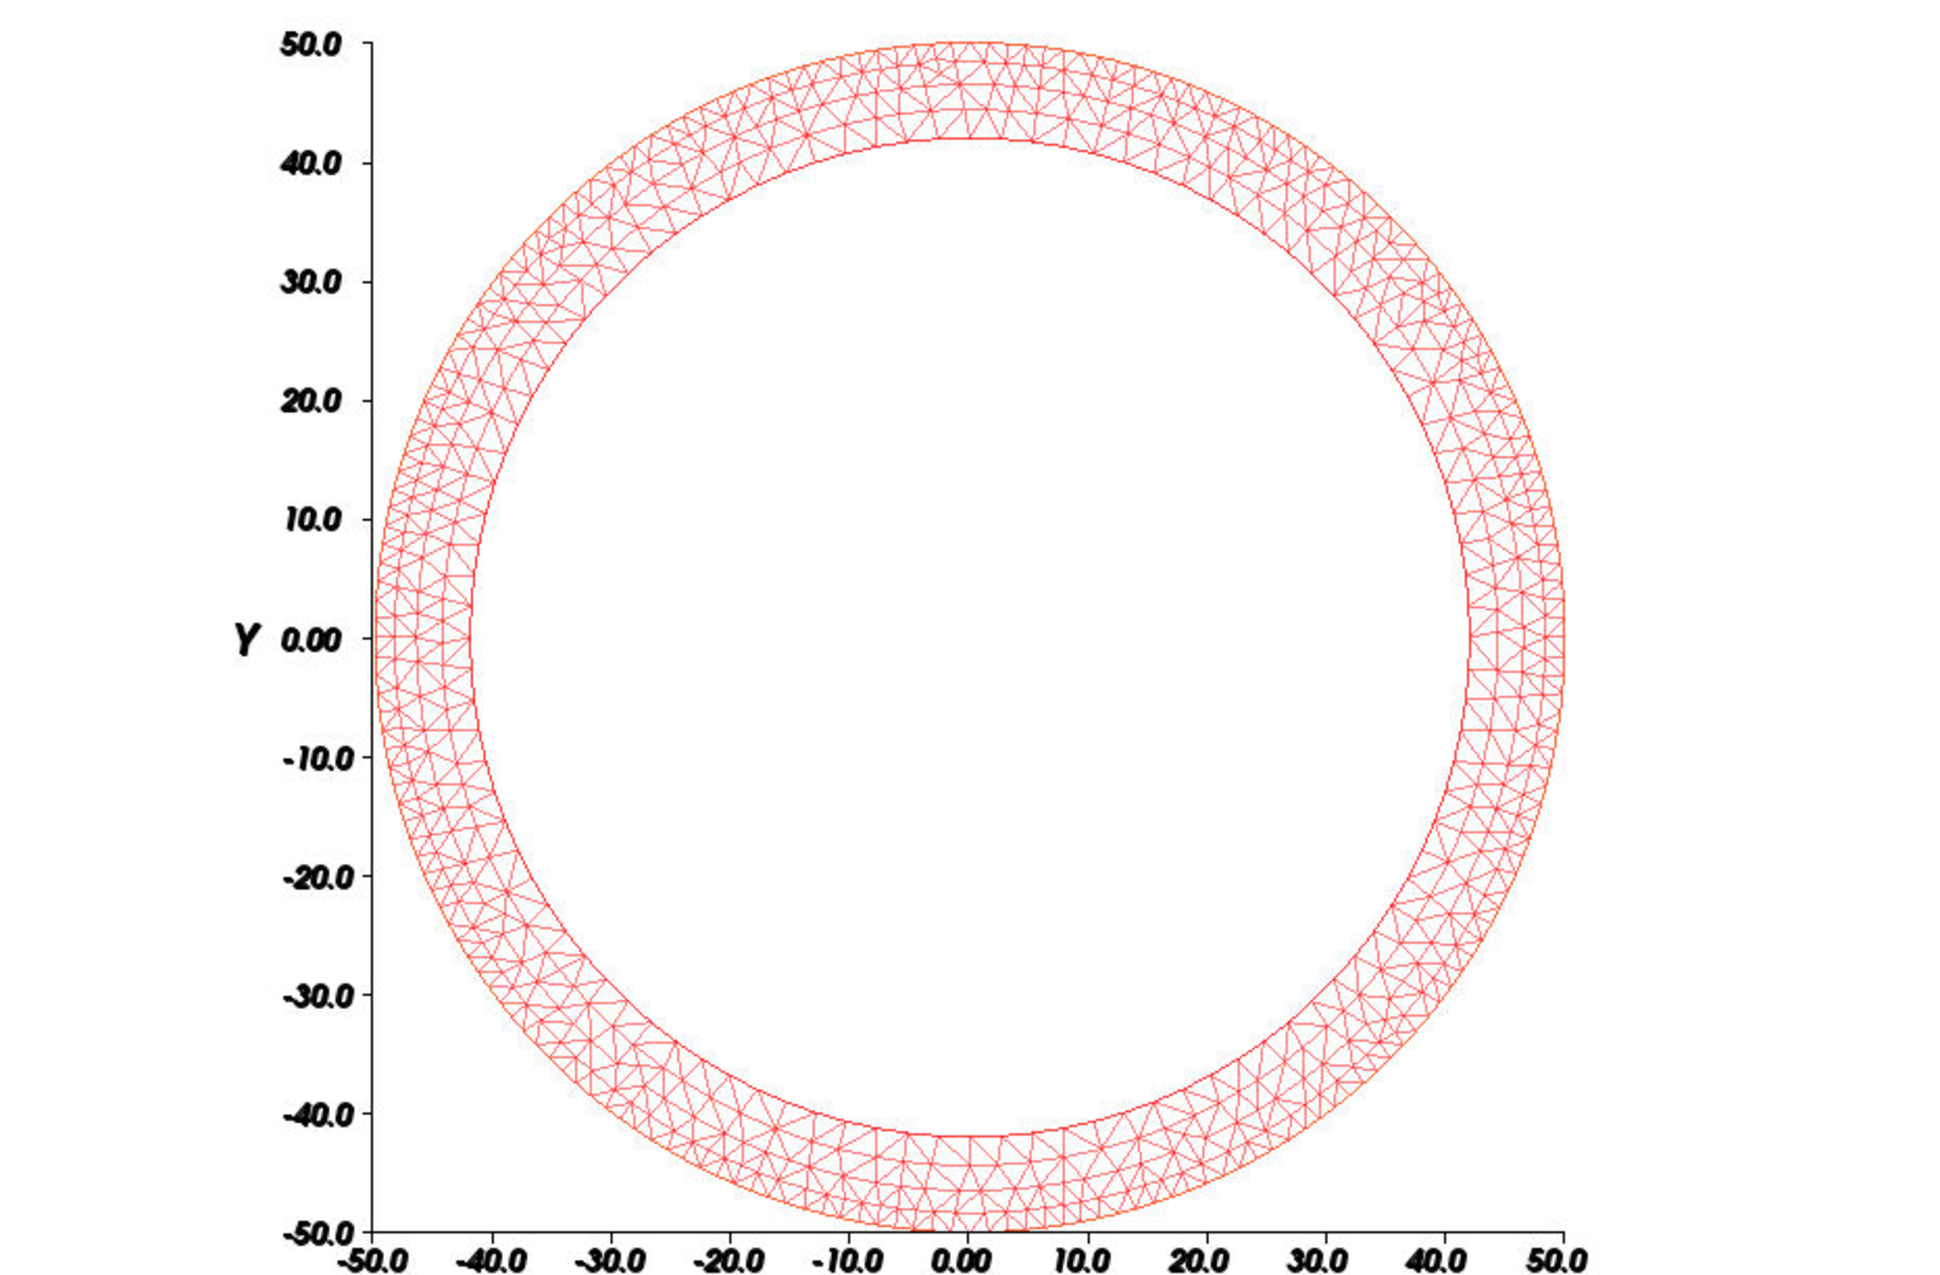
\includegraphics[width=0.7\textwidth]{paper/4-4-1.pdf}
\caption{Lưới khởi tạo của khuyên kim loại.}
\label{fig:exam41}
\end{figure}\\
Sự biến dạng của khuyên kim loại được biểu diễn như trong hình \ref{fig:exam42}:
\begin{figure}[http]
\centering
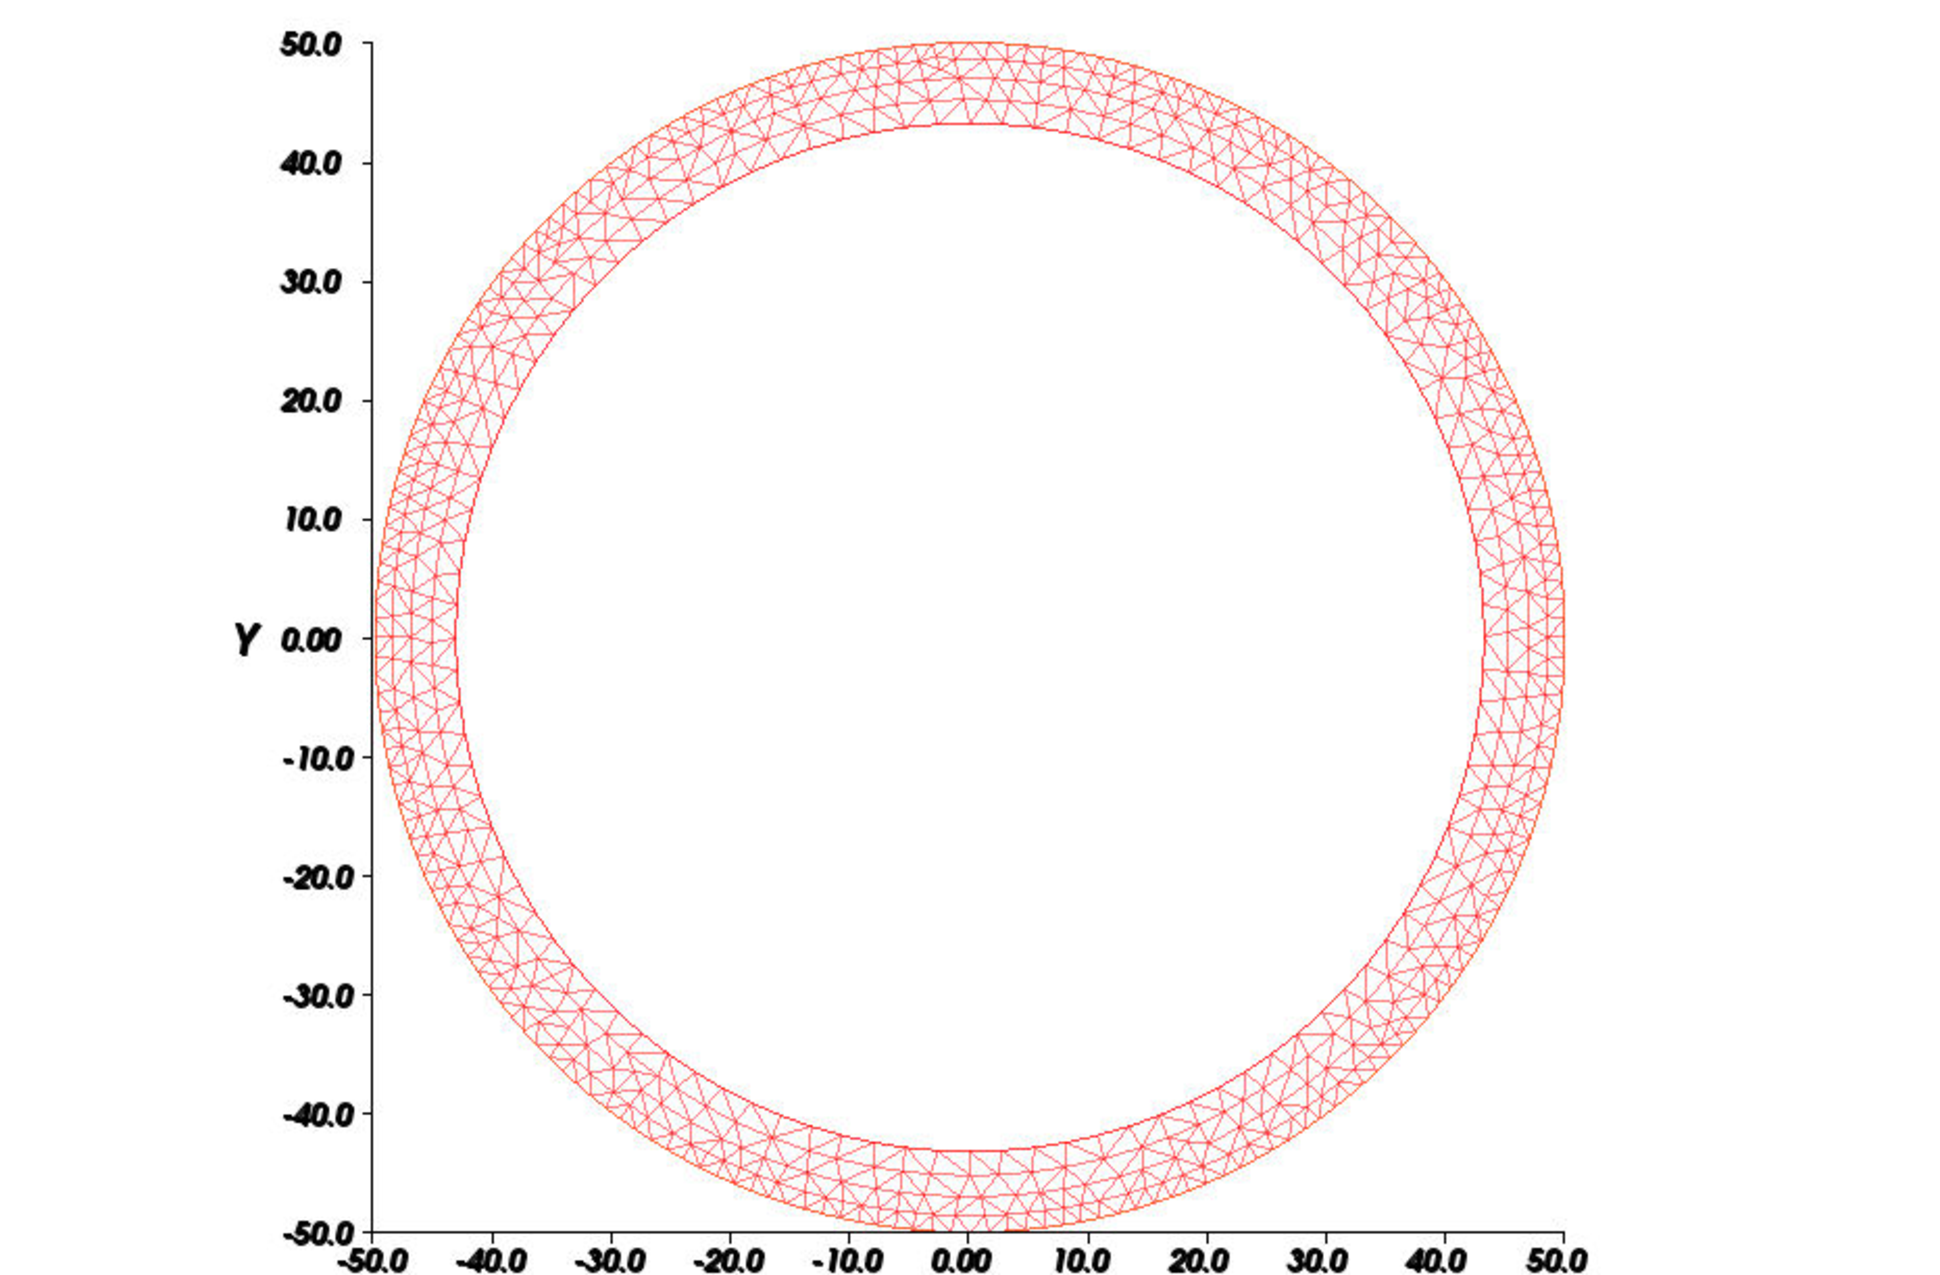
\includegraphics[width=0.7\textwidth]{paper/4-4-2.pdf}
\caption{Sự biến dạng của khuyên kim loại.}
\label{fig:exam42}
\end{figure}\\
Như đã nói ở trên, ta xét một ống kim loại. Có áp suất bên trong ống $p=1e3,E=2e5, v=0.3, r_i=40, r_e=50$ và ống có chiều dài $h=40$.\\
\begin{figure}[http]
\centering
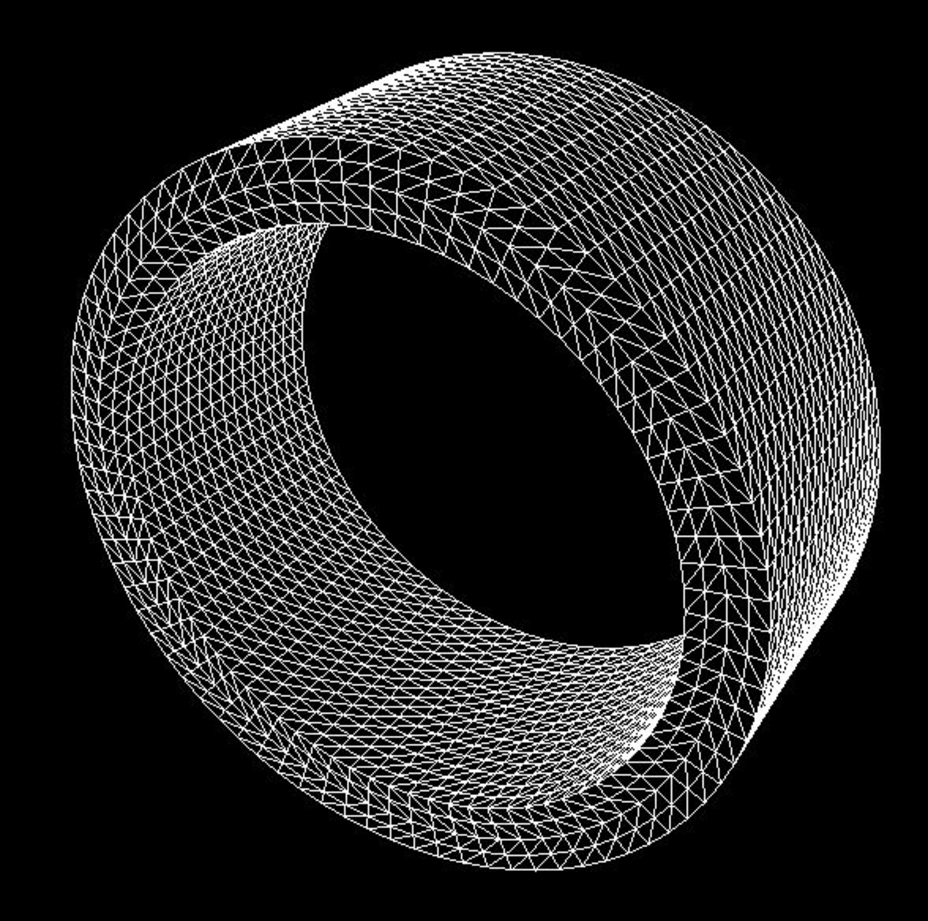
\includegraphics[width=0.6\textwidth]{paper/4-5.pdf}
\caption{Lưới khởi tạo của ống kim loại.}
\label{fig:exam50}
\end{figure}\\
Và các hình dưới đây cho thấy sự biến dạng của ống kim loại:
\begin{figure}[http]
\centering
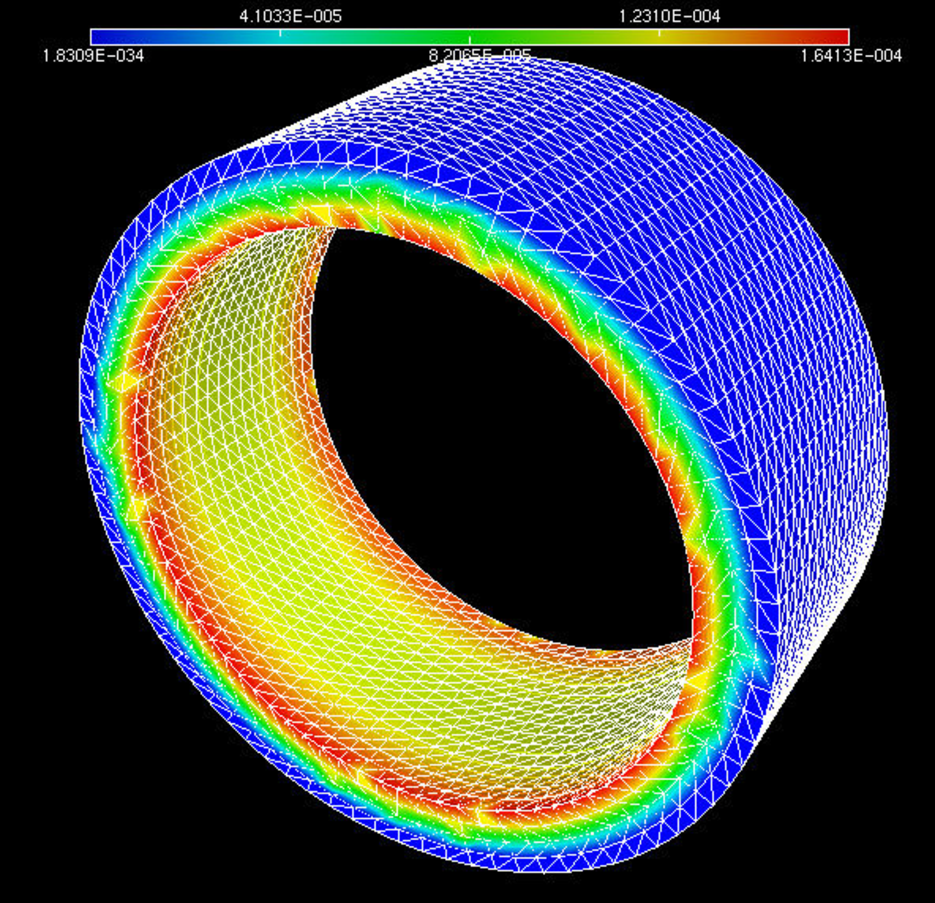
\includegraphics[width=0.6\textwidth]{paper/4-5-1.pdf}
\caption{Ống kim loại trước khi bị biến dạng.}
\label{fig:exam51}
\end{figure}\\
\begin{figure}[http]
\centering
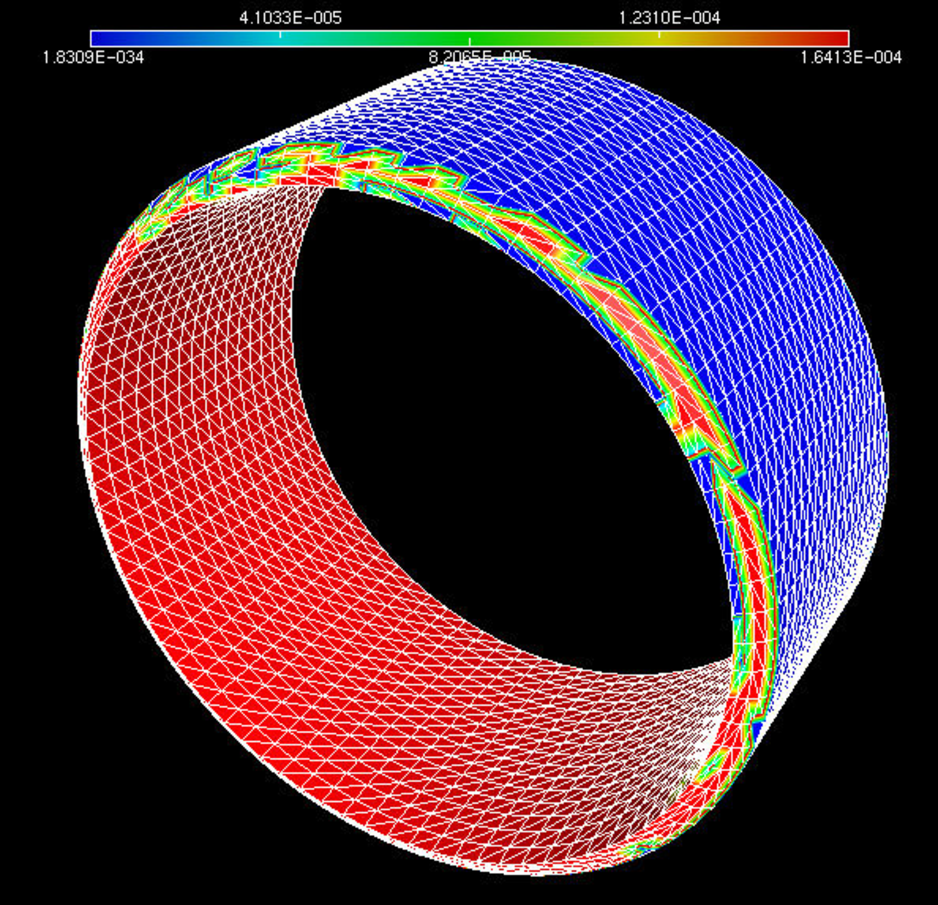
\includegraphics[width=0.6\textwidth]{paper/4-5-2.pdf}
\caption{Ống kim loại sau khi bị biến dạng.}
\label{fig:exam52}
\end{figure}\\

\section{Kết luận}
Trong chương này, ta đã trình bày chi tiết các bước xây dựng lược đồ giải số cho hệ phương trình biến dạng đàn hồi. Cụ thể, nội dung chương \ref{Chapter1} đã giải quyết những vấn đề sau:
\begin{itemize}
\item Phát biểu bài toán biến dạng đàn hồi.
\item Áp dụng phương pháp phần tử hữu hạn rời rạc hóa không gian, từ đó xây dựng bài toán rời rạc và hệ phương trình đại số tương ứng.
\item Trình bày các ví dụ giải số minh họa.
\end{itemize}

%----------------------------------------------------------------------------------------
